\section{Evaluation}\label{sec:results}
This is result section.

\subsection{Micro-benchmark for FMCW}

    - Different distance measurement accuracy

    - Wall orientation w.r.t path of the phone accuracy (Showing one gets perpendicular distance)
 
    - Resolution of distance measurement accuracy

    - Reflector size

   - Impact of phone height (peaks from ceiling + floor) and phone holding pattern
   
\subsection{Dead-reckoning based estimation}
   - Path profiling error (accelerometer + gyro)
   \begin{figure}[h!t]
   \center{
   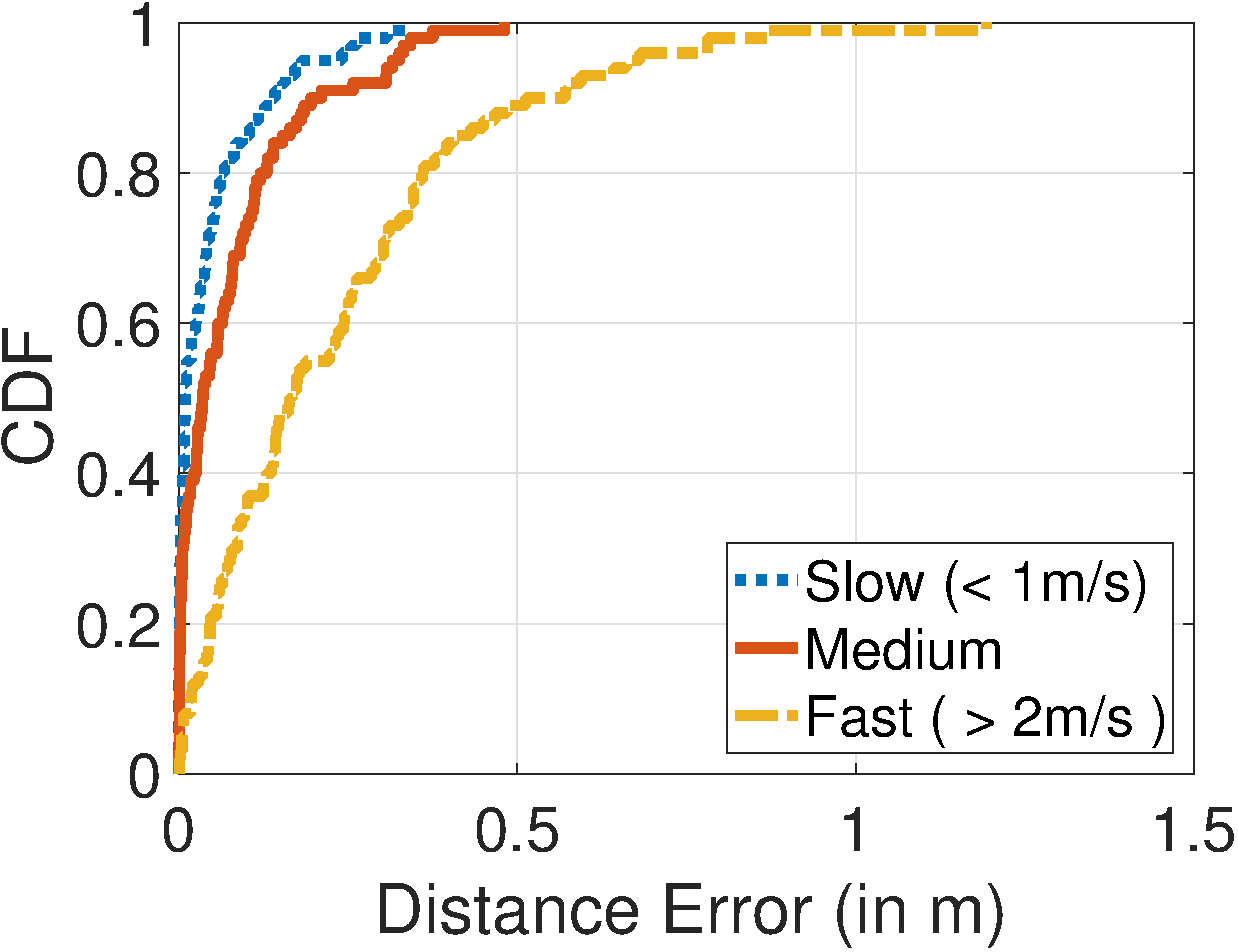
\includegraphics[width=\columnwidth]{figs/cdf-localization-deadreckoning.pdf}
   \caption{Dead-reckoning based distance estimation error.}
   \label{fig:with_dead_reckoning}
   }
   \end{figure}
   
\subsection{Single wall Contour}

  - Different shape Straight and Angled
 
   - Also need to try more shapes and sizes

\subsection{Multi wall Contour}

  Corner detection accuracy (False positive rate)
  
  Closed Intersections
   
  - Different angles
 
  - Different sized walls in intersection
  
  - Direction association accuracy (If you are moving along a straight line and you have one wall in right or left side. How do you know which side is your wall ?)
  
  Semi-Closed intersections
  
\begin{figure}[h!t]
\center{
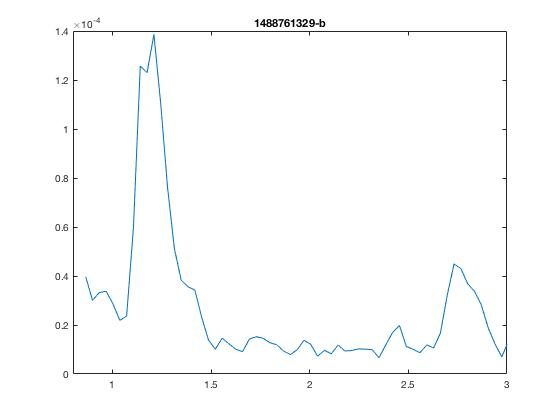
\includegraphics[width=\columnwidth]{figs/anechoic/8by8.jpg}
\caption{FMCW based and peak detection for distance measurement}
\label{fig:fmcw_distance}
}
\end{figure}

\begin{figure}[h!t]
\center{
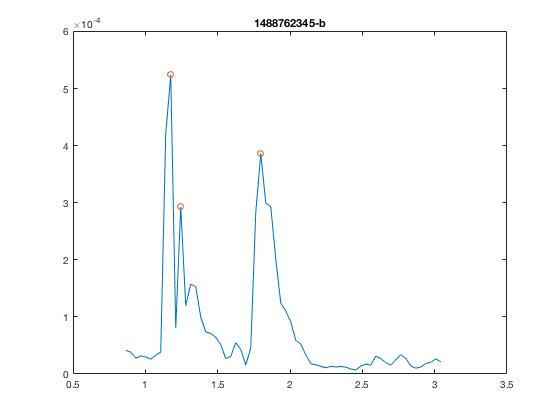
\includegraphics[width=\columnwidth]{figs/anechoic/with_floor_60_s2.jpg}
\caption{With floor}
\label{fig:with_floor}
}
\end{figure}

\begin{figure}[h!t]
\center{
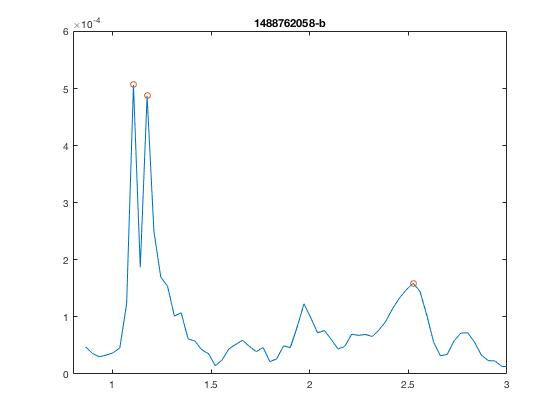
\includegraphics[width=\columnwidth]{figs/anechoic/without_floor_60.jpg}
\caption{Without floor}
\label{fig:without_floor}
}
\end{figure}

\subsection{Multi wall Contour with clutter}

Sensitivity to surrounding small objects by trying to add different sizes small objects at different locations to see if you can effectively filter them out 